\documentclass[a4paper,slidestop,xcolor=pst,blue]{beamer}

\usepackage{beamerthemesplit}
\usepackage[utf8]{inputenc}
\usepackage[spanish]{babel}
\usepackage{graphicx}
\usepackage{pstricks} % PSTricks package
\usepackage{setspace}
\usepackage{multirow}
\usepackage{listings}
\usepackage{pgfpages}
\usepackage{hyperref}
\usepackage{etoolbox}
\usepackage{epstopdf}

\makeatletter
\patchcmd{\beamer@sectionintoc}{\vskip1.5em}{\vskip0.5em}{}{}
\makeatother

\setbeamercovered{dynamic}
\setcounter{tocdepth}{2}
\setbeamercolor{frametitle}{fg=black,bg=white}
\setbeamercolor{section in toc shaded}{fg=black}
\setbeamercolor{section in toc}{fg=red}
\setbeamercolor{subsection in toc shaded}{fg=black}
\setbeamercolor{subsection in toc}{fg=red}
\setbeamerfont{section in toc}{size=\small}
\setbeamerfont{subsection in toc}{size=\small}
\setbeamertemplate{section in toc shaded}[default][99]
\setbeamertemplate{subsection in toc shaded}[default][99]

\AtBeginSection[]
{\begin{frame}[c]
  \frametitle{Índice}
	\tableofcontents[currentsection,
        sectionstyle=show/shaded,
        subsectionstyle=hide]
\end{frame}}

\AtBeginSubsection[]
{\begin{frame}[c]
	\frametitle{Índice}
	\tableofcontents[
  		currentsection,
  		sectionstyle=shaded/shaded,
  		currentsubsection,
  		subsectionstyle=show/shaded/hide
		]
\end{frame}}

\setbeamercolor{frametitle}{fg=black,bg=white}

\setbeamertemplate{frametitle}{
	\begin{centering}
		\insertframetitle
		\par
	\end{centering}
}

\usetheme[secheader]{Boadilla} 

\title[Introducci�n a las Arq. Empresariales]{Introducci�n a las Arquitecturas Empresariales}

\author[P. S�nchez]{\alert{Pablo S�nchez}}

\institute[IIE]{
		   Dpto. Ingenier�a Inform�tica y Electr�nica \\
		   Universidad de Cantabria \\
		   Santander (Cantabria, Espa�a) \\
		   \texttt{p.sanchez@unican.es}
}

\date{}

\begin{document}

\begin{frame}[c]
	\titlepage
	\begin{columns}
		\column{0.50\linewidth}
			\centering
    		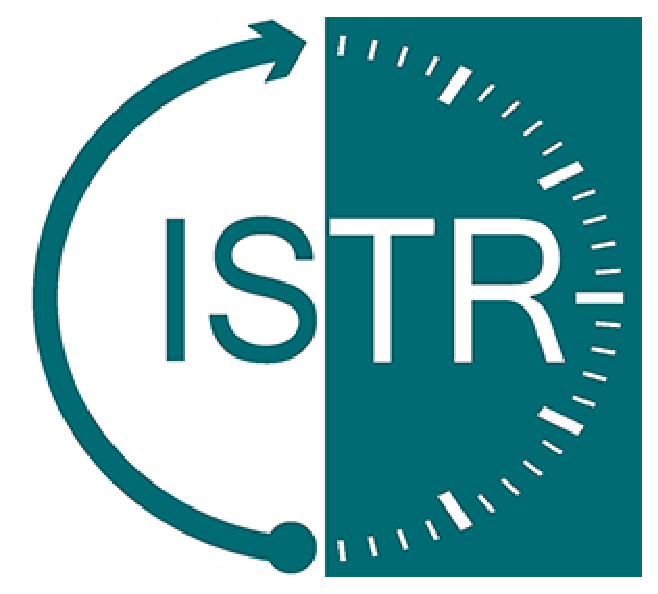
\includegraphics[width=.28\textwidth,keepaspectratio=true]{images/istr.eps}
		\column{0.50\linewidth}
			\centering
			
\includegraphics[width=.25\textwidth,keepaspectratio=true]{images/uc.eps}
	\end{columns}
\end{frame}

\begin{frame}[c]
    \frametitle{\alert{Advertencia}}
    \begin{center}
        Todo el material contenido en este documento no constituye en modo alguno una obra de referencia o apuntes oficiales mediante el cual se puedan preparar las pruebas evaluables necesarias para superar la asignatura. \ \\
        \ \\
        Este documento contiene exclusivamente una serie de diapositivas cuyo objetivo es servir de complemento visual a las actividades realizadas en el aula para la transmisi�n del contenido sobre el cual versar�n las mencionadas pruebas evaluables.  \ \\
        \ \\
        Dicho de forma m�s clara, \alert{estas transparencias no son apuntes y su objetivo no es servir para que el alumno pueda preparar la asignatura.}
    \end{center}
\end{frame}

\section{Introducci�n}

\subsection{Objetivos y Bibliograf�a}

\begin{frame}[c]
    \frametitle{Objetivos del Tema}
    \begin{enumerate}[<+->]
         \item Comprender en profundidad cu�les son las responsabilidades de la capa de dominio.
         \item Conocer los principales patrones relacionados con el desarrollo de una capa de dominio.
         \item Conocer las ventajas e inconvenientes del patr�n \emph{Domain Model}.
         \item Ser capaz de aplicar el patr�n \emph{Domain Model}.
         \item Ser capaz de aplicar los principios de \emph{Domain-Driven Design}.
    \end{enumerate}
\end{frame}

\begin{frame}[c]
    \frametitle{Bibliograf�a}
    \begin{thebibliography}{1}

        \bibitem[Fowler, 2002]{Fowler2002x}
        Fowler, M. (2002).
        \newblock {\em {Patterns of Enterprise Application Architecture}}.
        \newblock Addison-Wesley.

        \bibitem[Evans, 2013]{Evans2003}
        Evans, E. J. (2003).
        \newblock {\em {Domain-Driven Design}}.
        \newblock Addison-Wesley.

        \bibitem[Esposito and Saltarello, 2014]{Esposito2014}
        Esposito, D. and Saltarello, A. (2014).
        \newblock {\em {Microsoft .NET - Architecting Applications for the
          Enterprise}}. 2� Ed..
        \newblock Microsoft Press

    \end{thebibliography}
\end{frame}

\subsection{Contexto: Capa de Dominio}

\begin{frame}[c]
    \frametitle{Capa de Dominio}
\end{frame}

\begin{frame}
    \frametitle{Responsabilidades de la Capa de Dominio}
    %% Copiar y pegar del Tema 1
\end{frame}

\section{Patrones para la Capa de Dominio}

\subsection{Table Module}

\begin{frame}
    \frametitle{Table Module (deprecated)}
    %% Copiar y pegar del Tema 1
\end{frame}

\subsection{Transaction Script}

\begin{frame}
    \frametitle{Transaction Script}
    %% Copiar y pegar del Tema 1
\end{frame}

\subsection{Domain Model + Service Layer}

\section{Domain-Driven Design}

\section{Sumario y Conclusiones}

\end{document}
